%File: formatting-instructions-latex-2024.tex
%release 2024.0
\documentclass[letterpaper]{article} % DO NOT CHANGE THIS
\usepackage{aaai24}  % DO NOT CHANGE THIS
\usepackage{times}  % DO NOT CHANGE THIS
\usepackage{helvet}  % DO NOT CHANGE THIS
\usepackage{courier}  % DO NOT CHANGE THIS
\usepackage[hyphens]{url}  % DO NOT CHANGE THIS
\usepackage{graphicx} % DO NOT CHANGE THIS
\urlstyle{rm} % DO NOT CHANGE THIS
\def\UrlFont{\rm}  % DO NOT CHANGE THIS
\usepackage{natbib}  % DO NOT CHANGE THIS AND DO NOT ADD ANY OPTIONS TO IT
\usepackage{caption} % DO NOT CHANGE THIS AND DO NOT ADD ANY OPTIONS TO IT
\frenchspacing  % DO NOT CHANGE THIS
\setlength{\pdfpagewidth}{8.5in}  % DO NOT CHANGE THIS
\setlength{\pdfpageheight}{11in}  % DO NOT CHANGE THIS
%
% These are recommended to typeset algorithms but not required. See the subsubsection on algorithms. Remove them if you don't have algorithms in your paper.
\usepackage{algorithm}
\usepackage{algorithmic}

%
% These are are recommended to typeset listings but not required. See the subsubsection on listing. Remove this block if you don't have listings in your paper.
\usepackage{newfloat}
\usepackage{listings}
\DeclareCaptionStyle{ruled}{labelfont=normalfont,labelsep=colon,strut=off} % DO NOT CHANGE THIS
\lstset{%
	basicstyle={\footnotesize\ttfamily},% footnotesize acceptable for monospace
	numbers=left,numberstyle=\footnotesize,xleftmargin=2em,% show line numbers, remove this entire line if you don't want the numbers.
	aboveskip=0pt,belowskip=0pt,%
	showstringspaces=false,tabsize=2,breaklines=true}
\floatstyle{ruled}
\newfloat{listing}{tb}{lst}{}
\floatname{listing}{Listing}
%
% Keep the \pdfinfo as shown here. There's no need
% for you to add the /Title and /Author tags.
\pdfinfo{
/TemplateVersion (2024.1)
}


\usepackage{makecell}

% DISALLOWED PACKAGES
% \usepackage{authblk} -- This package is specifically forbidden
% \usepackage{balance} -- This package is specifically forbidden
% \usepackage{color (if used in text)
% \usepackage{CJK} -- This package is specifically forbidden
% \usepackage{float} -- This package is specifically forbidden
% \usepackage{flushend} -- This package is specifically forbidden
% \usepackage{fontenc} -- This package is specifically forbidden
% \usepackage{fullpage} -- This package is specifically forbidden
% \usepackage{geometry} -- This package is specifically forbidden
% \usepackage{grffile} -- This package is specifically forbidden
\usepackage{hyperref} % -- This package is specifically forbidden
\usepackage{cleveref}
%\usepackage{navigator} % -- This package is specifically forbidden
% (or any other package that embeds links such as navigator or hyperref)
% \indentfirst} -- This package is specifically forbidden
% \layout} -- This package is specifically forbidden
% \multicol} -- This package is specifically forbidden
% \nameref} -- This package is specifically forbidden
% \usepackage{savetrees} -- This package is specifically forbidden
% \usepackage{setspace} -- This package is specifically forbidden
% \usepackage{stfloats} -- This package is specifically forbidden
% \usepackage{tabu} -- This package is specifically forbidden
% \usepackage{titlesec} -- This package is specifically forbidden
% \usepackage{tocbibind} -- This package is specifically forbidden
% \usepackage{ulem} -- This package is specifically forbidden
% \usepackage{wrapfig} -- This package is specifically forbidden
% DISALLOWED COMMANDS
\nocopyright % -- Your paper will not be published if you use this command
% \addtolength -- This command may not be used
% \balance -- This command may not be used
% \baselinestretch -- Your paper will not be published if you use this command
% \clearpage -- No page breaks of any kind may be used for the final version of your paper
% \columnsep -- This command may not be used
% \newpage -- No page breaks of any kind may be used for the final version of your paper
% \pagebreak -- No page breaks of any kind may be used for the final version of your paperr
% \pagestyle -- This command may not be used
% \tiny -- This is not an acceptable font size.
% \vspace{- -- No negative value may be used in proximity of a caption, figure, table, section, subsection, subsubsection, or reference
% \vskip{- -- No negative value may be used to alter spacing above or below a caption, figure, table, section, subsection, subsubsection, or reference

\setcounter{secnumdepth}{0} %May be changed to 1 or 2 if section numbers are desired.

% The file aaai24.sty is the style file for AAAI Press
% proceedings, working notes, and technical reports.
%

% Title

% Your title must be in mixed case, not sentence case.
% That means all verbs (including short verbs like be, is, using,and go),
% nouns, adverbs, adjectives should be capitalized, including both words in hyphenated terms, while
% articles, conjunctions, and prepositions are lower case unless they
% directly follow a colon or long dash
\title{Exploring Transformers for Answering Crossword Clues}
\author {
    Mike Chaberski
}
\affiliations {
    NYU Tandon School of Engineering\\
    mac937@nyu.edu
}

\begin{document}

\maketitle

\begin{abstract}
    The design and implementation of transformer neural network models for answering crossword puzzle clues is explored herein.
    A word-generating model and a letter-generating model are defined and tuned based on training results.
    The models are evaluated relative to a baseline non-neural-network algorithm.
    Model definition, training, and evaluation code is available at \url{https://github.com/mike10004/csgy6953-fp1}.
\end{abstract}

\begin{NoHyper}

\section{Introduction}
\label{sec:intro}

Humans solve crossword puzzles with a variety of skills, including language facility, trivia knowledge, and lateral thinking.
Transformer models show adeptness at mining training data for obsfuscated connections among samples in tasks such as language translation.
Therefore, it is plausible that a transformer trained on crossword clue-answer pairs could discover approximations of the
skills required to suggest correct answers to crossword clues.

This work explores the design and implementation of transformer models trained to answer crossword clues.
Two models are developed, one that suggests a single word given an input clue, and one that suggests a
sequence of letters.
The definintion and training of these models is discussed below.
The letter model requires some additional engineering beyond the training step, as
additional considerations must be contemplated for the generator component that produces
sequences of letters in response to a clue.

\section{Related Work}
\label{sec:related}

The intuition behind the use of transformers for answering clues is the robust performance of transformer models at
the machine translation task~\cite{vaswani2017}.
Mapping crossword clues to answers is a sequence-to-sequence translation task, with the caveats that the source
sequences (clues) are generally terse and often contain misdirection, and the target sequences (answers) are
generally very short relative to the length of the source sequence.

The end-to-end task of solving a complete crossword grid is notably tackled in~\citealp{wallace2022automated},
which produced an algorithm that outperformed humans at the American Crossword Puzzle Tournament in 2021.
The clue-answering component is a bi-encoder QA model designed to be used iteratively to solve harder clues
given probable letters from easier crossing answers.
Contemporaneous work from~\citealp{kulshreshtha2022across} suggests end-to-end crossword grid-solving
as a benchmark Natural Language Processing algorithm capabilities.

The task this study investigates is limited to answering clues (as opposed to populating a grid),
which is a type of reverse-dictionary problem addressed in~\citealp{zhang2019multichannel}.
The authors develop the \textit{MultiRD} model, a bidirectional LSTM model with a ``multi-channel'' approach that
integrates linguistic analysis (e.g.~morphemes, lexemes, and semantic units).

A statistical approach to answering clues is implemented in~\citealp{baselinesolver}.
That work does not train a model on a clue-answer database, but instead uses word embeddings to maximize similarity to
clues in a database, and selects answers based on best-matching clues.
That method is the baseline against which our model results are compared in the test phase.

\begin{figure*}
\centering
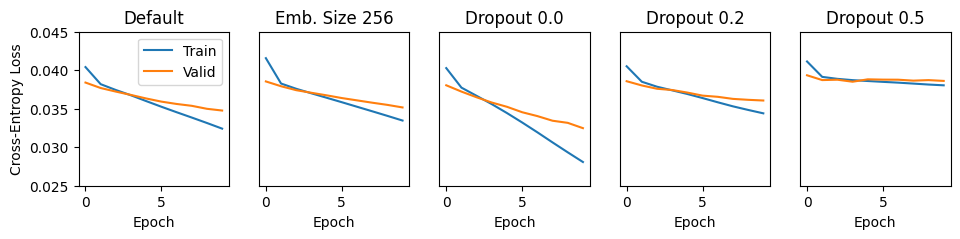
\includegraphics[width=0.8\textwidth]{fig-onemark-loss-all}
\caption{\textbf{Word model} training and validation loss curves under varying hyperparameters.}
\label{fig:onemark-loss}
\end{figure*}

\begin{figure*}
\centering
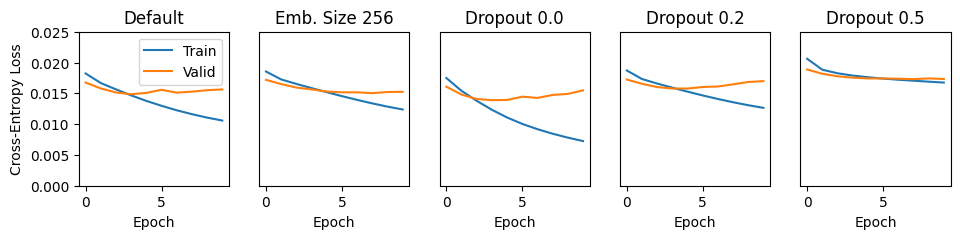
\includegraphics[width=0.8\textwidth]{fig-charmark-loss-all}
\caption{\textbf{Letter model} training and validation loss curves under varying hyperparameters.}
\label{fig:charmark-loss}
\end{figure*}

\section{Dataset}
\label{sec:dataset}

A modified version of the dataset from~\citealp{kulshreshtha2022across} is used for training and evaluation.
The modified dataset contains only single-word answers and does not contain cross-referential clues (e.g.~``See 46-Across'').
The training set has 320K clue-answer pairs, and there are about 55K in the validation and test sets.

\section{Model Selection}
\label{sec:model}

Model structure and training code was adapted from a transformer implementation for sequence to sequence translation~\cite{chegde2022}.
A custom generator component was developed to support ranked answer suggestions.
Default hyperparameters for each model were either adopted from~\citealp{vaswani2017} or inherited from the upstream codebase.
Adopted hyperparameters include:

\begin{itemize}
\item 8 attention heads;
\item embedding size 512;
\item 3 encoder layers and 3 decoder layers;
\item sinusoidal positional encoding;
\item feed-forward network dimension 512;
\item Adam optimizer~\cite{kingma2017adam} with $\beta_1 = 0.9$, $\beta_2 = 0.98$, and $\epsilon = 10^{-9}$; and
\item dropout rate 0.1.
\end{itemize}

The use of cross-entropy for the loss function and learning rate of $10^{-4}$ were inherited from the upstream codebase.
Learning rates of greater magnitude were tested but in each case the loss did not trend toward convergence.
The batch size of 128 was likewise taken from the upstream codebase.

Models were trained for 10 epochs.
Initial results of training both the word model and the letter model showed a propensity for overfit.
As such, different methods of preventing overfit by varying hyperparameters were attempted.
These included regularization by varying dropout rates and reducing model dimensionality by decreasing embedding size to 256.
A dropout rate of zero was also tested to determine whether dropout was actually appropriate for the task.

\subsection{Word Model}
\label{subsec:word}

Training and validation loss curves for the word model are shown in~\autoref{fig:onemark-loss}.
All of the curve pairs show undesirable characteristics.
In the case of the default parameters and the reduced dimensionality, growing divergence between training and validation loss is evident.
In the case of dropout, at a dropout rate of zero, the model achieves lower validation loss than under the default rate of 0.1. At greater dropout rates, the loss converges  early at a loss value greater than under the default rate.

The model trained under default parameters and the model trained with zero dropout show similar overfit propensity, but the zero-dropout model achieves lower loss.
Thus the zero-dropout model, with 110 million trainable parameters, was selected as the optimal word model for subsequent consideration.

\subsection{Letter Model}
\label{subsec:letter}

Training and validation loss curves for the letter model are shown in~\autoref{fig:charmark-loss}.
As with the word model, all of the curve pairs show undesirable characteristics.
Under the default parameters, the model shows substantial overfit, with the validation loss on an increasing trajectory at later epochs.
Overfit is also evident in the loss curves of the model with reduced dimensionality, but that model shows a better overall trend, which aligns with the intuition that the small target token space of the letter model would be accommodated better by a lower-dimension model.

Examination of the loss curves for models trained under varying dropout rates shows that a dropout rate of zero induces substantial overfit and an increasing validation loss trend, similar to the default model but magnified.
At dropout rate 0.5 there is no evidence of overfit, but the loss appears to have converged early.

The reduced overfit but greater minimum validation loss (0.0173) of the 0.5-dropout model was weighed against the greater overfit and minimum validation loss of 0.0152.
The reduced-dimensionality model, with 25 million trainable parameters, was selected as optimal for subsequent consideration.

\section{Generator Strategy}
\label{sec:generator}

Given a sequence-to-sequence transformer model, a sequence generator is the component that accepts as input a source sequence and an empty or partial output sequence and produces the next element of the output sequence. The generator is iteratively applied to produce a complete sequence. For both the word and letter models, the source sequence is a clue. The word model generator produces a sequence of words and the letter model generator produces a sequence of letters.

For each input, the generator produces an array of values corresponding to possible next tokens. The values are relative measures of likelihood. Our generator implementation applies the softmax function to these values to map them to a probability distribution. (This is the default behavior of the implementation, but other mappings are supported.)

To produce a list of candidate answers for a given clue, beam search is performed. In beam search, the tree of sequence possibilities is traversed and the resulting answers are ranked by their cumulative probability. The cumulative probability of an answer is the product of the probabilities of the constituent sequence elements (words or letters, depending on the model).

At each node of the tree, the possible next tokens are considered in order of probability, descending, up to a limit parameter.
We identify a given tree search strategy by the sequence of these limit parameters, so a strategy that looks at the top 10 tokens, then top 5, then top 3, would be identified by the string L10-5-3.
For brevity, the last number in the identifying sequence is assumed for all subsequent decision nodes, so a strategy that considers 2 tokens at every node is identified by the string L2. (Because the sequences the word model may generate are at most one token, only the L100 strategy is evaluated for the word model.)

Performance under different strategies for generating answers is shown in~\autoref{fig:onemark-acc-by-strat} and~\autoref{fig:charmark-acc-by-strat} by evaluating their performance in producing correct answers.
Because this generator strategy is exponential in runtime by nature, evaluation was performed on a random 1000-pair subset of the validation set.
The letter model was evaluated on a subset that contains only answers up to 5 letters in length.
Performance is measured by calculating the percentage of correct answers at incremental ranks.
For example, the accuracy at rank 10 is the percentage of clue-answer pairs for which the correct answer is among the top 10 candidate answers.

\begin{figure}
\centering
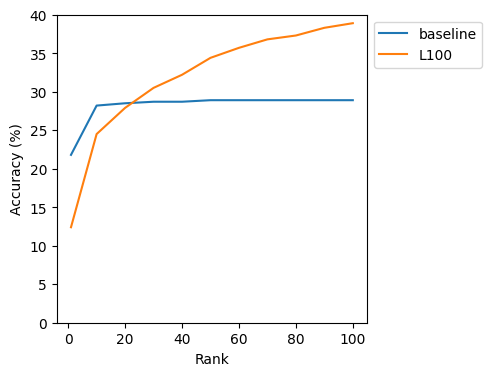
\includegraphics[width=0.95\columnwidth]{fig-onemark-acc-by-strat}
\caption{\textbf{Word model} accuracy by generator strategy.}
\label{fig:onemark-acc-by-strat}
\end{figure}

\begin{figure}
\centering
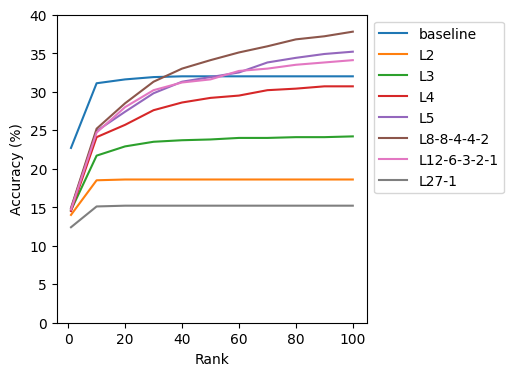
\includegraphics[width=0.95\columnwidth]{fig-charmark-accuracy-default-tmp}
\caption{\textbf{Letter model} accuracy by generator strategy.}
\label{fig:charmark-acc-by-strat}
\end{figure}

Both models are outperformed by the baseline at rank less than 20.
The word model shows a generally positive trend, and the fact that it is achieving near 40\% accuracy at rank 100, when the size of the answer set is about 50K, shows that the model is indeed learning effectively.

With respect to the letter model, the lower-order strategies do not achieve significant accuracy, and their accuracy with respect to rank has a low upper bound because the search space is only $k^5$ (where $k$ is the number of letters).
The higher-order strategies achieve some success,  outperforming the baseline at ranks above 30.
Strategies that are broadly less greedy, meaning they consider more tokens at greater depths in the search tree, appear to outperform greedier strategies with greater initial degrees.
In particular, strategy L5 performs quite well for its low-degree search space, and its efficiency recommends it as the optimal strategy for subsequent evaluation in the test phase.

\section{Results}
\label{sec:results}

For the test phase, subsets of the test set were constructed, with 10K pairs
for the word model and 1K pairs for the letter model.
The letter model set includes only pairs with answers of at most 5 letters.
The results are shown in~\autoref{fig:test-acc}.

\begin{figure}
\centering
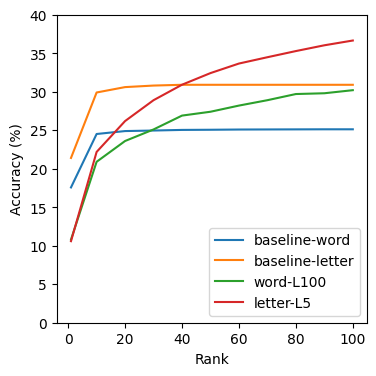
\includegraphics[width=0.75\columnwidth]{fig-test-acc}
\caption{Accuracy of selected models and strategies on test subsets.}
\label{fig:test-acc}
\end{figure}

The performance difference in the baselines is presumably because clues with
shorter answers are more easily matched by the baseline algorithm.
The word model outperforms the baseline at ranks above 20, and the letter model
outperforms the baseline at ranks above 40.

\section{Conclusion}
\label{sec:conclusion}

The models achieve success in outperforming the baseline, but the baseline is a low bar.
Comparison to the MultiRD model or even a basic Word2Vec-based algorithm that contemplates semantic content would provide a better gauge of relative performance.
(Performance of the MultiRD model could not be reproduced at the accuracy level reported by~\citeauthor{zhang2019multichannel}, so it was deemed unfair to include as a baseline herein.)

The initial objectives from the project proposal included attempting to utilize constraints such as target sequence length and known letters, but given the complexity of the initial tasks of model training and generator implementation, adding those objectives would have broadened the scope greatly, resulting in more cursory investigation of the core methods that were explored herein.
Use of positional encoding to influence output sequence length~\cite{takase2019positional} seems like a promising way to achieve better accuracy at lower ranks.
The known-letters constraint can be seen as a specific instance of the general problem of unmasking partially-masked
sequences given an input context, which is tackled by~\citealp{raffel2023exploring}, among others.

The fundamental model training task proved difficult.
It is possible that propensity toward overfit is an inherent characteristic of crossword clue/answer datasets, relative
to datasets for language translation on which transformers have shown robustness.
Clue-answer pairs are inherently asymmetric in terms of sequence length, whereas language-to-language pairs are more balanced.
This also points toward consideration of alternative positional encodings for the answer sequences in the letter model;
given their short length, perhaps a sinusoidal encoding is not appropriate.
(Tests that completely removed the letter model's positional encoding from the target sequence were performed, but the results were poor.)
\citeauthor{kulshreshtha2022across} claim that no major transformer architecture supports character-level outputs, so
this was likely a more complex task than initially assumed.

While reducing model dimensionality and increasing dropout were attempted to introduce regularization, other
techniques, such as data augmentation (perhaps by randomly masking some tokens in the clue sequences) are worth trying.
Scheduling learning rate adjustments differently is also worthy of investigation; \citeauthor{vaswani2017} schedule the
learning rate with a warmup period and gradual decrease.
They train for many more epochs with a much larger dataset, but even for this dataset, non-constant learning rate
schedules are worthy of consideration.

Overall, the results herein show that the models did learn effectively, though imperfectly.
Though there is conclusive evidence that the transformer architecture is optimal for the clue-answering task,
relative to other types of encoder-decoder models, several avenues of further research are promising.

\bibliography{aaai24}

\end{NoHyper}

\end{document}
